%!tex root=./thesis.tex
\chapter{Radio Luminosity Functions}
\label{cha:rlfs}

% make James' picture of binary xid before partitioning and colour it with a value-ramped viridis.

% \section{Making Catalogues with Binary Cross-identification}
% \label{sec:rlfs-revisiting-cross-id}


% \section{FIRST paper...}

This chapter is based on my paper \emph{Radio Galaxy Zoo: Radio Luminosity Functions of Extended Sources}, by M. J. Alger, O. I. Wong, C. S. Ong, N. M. McClure-Griffiths, H. Andernach, L. Rudnick, S. S. Shabala, A. F. Garon, J. K. Banfield, A. D. Kapi\'nska, R. P. Norris, and A. J. M. Thomson; to be submitted. Some minor changes have been made to match the rest of this thesis.\\

In \autoref{cha:cross-id}, we concluded that our machine learning cross-identification approach was sound in principle, but the small size and lack of morphological complexity in ATLAS prevented training a good classifier. To demonstrate this, we turned our attention to the Faint Images of the Radio Sky at Twenty Centimeters (FIRST) survey, which contained many more sources and many more morphologically complex sources due to its higher resolution and sample size. If cross-identification of this dataset was successful, we could use the resulting cross-identification catalogue to investigate statistical properties of radio galaxies at larger scales than previously possible. The object of interest would be the radio luminosity function (RLF), a statistical description of how common radio galaxies of various luminosities are throughout the universe. The RLF would be specific to only extended radio galaxies, and it is this class of galaxies that we would expect to maximally impact its local environment through direct, mechanical energy input.

In this chapter, we use a machine learning model trained on the Radio Galaxy Zoo citizen science project to cross-identify \ncomponents{} radio components of extended radio sources from FIRST with \nsources{} host galaxies observed in the mid-infrared from the All\emph{WISE} source catalogue. \nsourceszsp{} hosts have a spectroscopic redshift in the Sloan Digital Sky Survey (SDSS). This is the largest available sample of cross-identified extended radio sources to date at the time of writing. The large sample size allows us to estimate the RLF of extended radio galaxies and to further characterise the sample with fractional radio luminosity functions. The extended source RLF can be used to estimate the mechanical energy injected into the local environment of active galactic nuclei (AGN). We estimate from the observed radio emission that inferred extended radio jets from AGN contribute between $1.3 \times 10^{30}$ and $1.2 \times 10^{32}$~W~Mpc$^{-3}$ of mechanical energy to their environment throughout the low-redshift ($z < 0.6$) Universe. By further visual verification we also find \nnewgiants{} radio galaxies with projected size larger than 1~Mpc. Our results directly demonstrate the impact that automated machine learning methods could have on future wide-area radio surveys.

\section{Introduction} \label{sec:rlfs-intro}

Radio active galactic nuclei (AGN) are some of the most violent and energetic
objects in the Universe. Supermassive black holes at the centre of galaxies
can produce large, luminous radio jets that may feed lobes extending up to
megaparsec scales. As a vital part of galaxy evolution, we want to understand
how radio AGN interact with their host galaxies, in what kinds of galaxies
these AGN are found, and how these populations change over cosmic time.

Mechanical energy from AGN is needed to explain the star-formation history of galaxies throughout the Universe \citep[e.g.][]{raouf17agn,hardcastle20feedback}. The radio luminosity function (RLF) of extended radio sources would characterise the energy output of galaxies capable of significant energy impact into their local environment. The local RLF of primarily compact sources is estimated and
described in detail by \citet{mauch07rlf}, \citet{pracy16rlf} and
\citet{condon19rlf}, each with complete volume-limited samples. However, the RLF of extended radio sources has not been
characterised as a separate sample, because estimating this RLF would need a large number of extended sources with known
redshifts. Such redshifts are usually obtained by cross-matching the radio
sources with their host galaxies in the optical or infrared. While this
cross-matching is relatively straightforward for compact/unresolved sources,
and can therefore be automated \citep[e.g.][]{kimball08}, extended radio
emission may be complex and may not be co-located with the host galaxy.
Cross-identification of complex, extended sources is therefore usually done
manually, limiting the sample size.

Wide-area radio surveys like the Very Large Array Faint Images of the Sky at
Twenty Centimeters survey \citep[FIRST;][]{white97first} have led to
catalogues of hundreds of thousands of radio objects, most of which are
associated with radio AGN \citep{sadler02rlf}. While individual galaxy
properties vary significantly between galaxies, the large sample size of
such surveys allows us to examine reliable bulk statistics that may
tightly constrain models and theory of radio galaxy evolution and formation \citep{condon92radio}. With a
sufficiently large sample \citep[of size $N$ such that $N \gg
\sqrt{N}$;][]{condon91rlf} we can also divide the RLF into fractions based
on the physical properties of each galaxy. These \defn{fractional RLFs} show
how different physical processes comprise the luminosity distribution, and
can be used to investigate how these processes relate to the properties of
the AGN.

In this chapter we calculate the RLF for extended radio sources in FIRST. Throughout this chapter we define an \defn{extended radio source} as a collection of extended radio components with the same host galaxy, and following
\citet{banfield15} we define an \defn{extended radio component} as a radio
component which fulfils \autoref{eq:rgz-criterion}:
\begin{equation}
    \frac{S_{\mathrm{peak}}}{S_{\mathrm{int}}} < 1 - \frac{0.1}{\log_{10}(S_{\mathrm{peak}} / 1\ \mathrm{mJy})},
    \label{eq:rgz-criterion}
\end{equation}
where $S_{\mathrm{peak}}$ is the peak radio flux density and
$S_{\mathrm{int}}$ is the integrated radio flux density. We define \defn{radio components} as Gaussians fit to
radio emission, \defn{radio islands} as connected patches of radio emission
above a local $4\sigma$ value, and \defn{radio sources} as sets of radio
islands or components associated with the same galaxy. The radio flux density of a source is the sum of the flux densities of the components according to the FIRST catalogue. The \defn{(infrared)
host galaxy} of a radio source or component is defined as the infrared galaxy
associated with the radio emitter. A \defn{cross-identification} is an
association of a host galaxy with one or more radio components or islands. We
define \defn{candidate host galaxies} (or simply
\defn{candidates}) as infrared objects that are near a radio component on
the sky and thus may potentially be the host galaxy of that component.

Upcoming
radio surveys such as the Evolutionary Map of the Universe
\citep[EMU;][]{norris11} are expected to increase the number
of complex radio sources to around 7 million \citep{banfield15}. Manual, expert cross-identification for such surveys will be impractical. One way forward could be to ask non-expert volunteers for help with manual cross-identification, which is the approach taken by Radio Galaxy Zoo \citep[RGZ;][]{banfield15}. This is called \defn{citizen science} and has been employed successfully in many fields with large datasets \citep{marshall15citizen}. Even this approach is not sufficient for 7 million sources, though, with RGZ cross-identifying around 75~000 sources in four years. Machine
learning provides a potential pathway to obtaining useful physics from such
large samples.

In this chapter, we train a machine learning model based on \citet{alger18radio}, using RGZ as training data, and
use this model to automatically cross-identify \ncomponents{} radio components catalogued by FIRST. This results in \nsourceszsp{} sources
with spectroscopic redshifts. This is the largest available catalogue of
extended radio source cross-identifications. We call our catalogue
\defn{RGZ-extrapolated} or \defn{RGZ-Ex}. Due to our large sample size we are able to further divide the
source population by properties of the host galaxies. We refer to the trained machine learning model and the associated cross-identification algorithm jointly as \defn{binary cross-identification}, or \defn{BXID}. Note that there are two stages to our automated approach: first, we train BXID using an existing catalogue of cross-identified sources; second, we generate new cross-identifications for radio components not in the training catalogue. We refer to these stages as \defn{training} and \defn{prediction} respectively. Our data sources are described in \autoref{sec:rlfs-data}. Our approach is discussed in \autoref{sec:rlfs-method}. Radio luminosity functions of extended sources are presented in \autoref{sec:rlfs-rlf} and we discuss these functions in \autoref{sec:rlfs-discussion}.

Throughout this chapter we assume a flat $\Lambda$-CDM cosmology of \linebreak $H_0 =
69.3$~km~s$^{-1}$~Mpc$^{-1}$, $\Omega_m = 0.287$. These are the cosmological
parameters from the Nine-year Wilkinson Microwave Anisotropy Probe
\citep[WMAP9;][]{hinshaw13wmap9}.

\section{Data} \label{sec:rlfs-data}

In this section we describe how we obtain our training and prediction data. To enable the estimation of the extended RLF, we apply a number of selection criteria to the data which are shown in \autoref{fig:sankey-sources}.

    \subsection{RGZ} \label{sec:rlfs-rgz-data}

    RGZ is a citizen science project that aims to cross-identify complex radio sources with mid-infrared host galaxies with the help of volunteers. The first RGZ data release contains around 75~000 cross-identifications of a random subset of extended sources in FIRST with their host galaxies in All\emph{WISE}. For more details on RGZ see \citet{banfield15}. This catalogue has also been used in other machine learning contexts, including supervised learning for source aggregation \citep{wu19claran} and unsupervised learning methods \citep{galvin19som,ralph19ae}. We discard the RGZ sources without a host galaxy detected in All\emph{WISE} and use the remaining 41~446 sources for training.

    The RGZ catalogue only contains sources with at least 0.65 weighted volunteer agreement, equivalent to approximately 80 per cent reliability. This implicitly selects for less complex sources, since the volunteer agreement is a proxy for the difficulty of cross-identifying a source (Wong et al. in prep).

    \subsection{FIRST} \label{sec:rlfs-first-data}

    We use radio imagery and select radio components from the FIRST survey and associated catalogue respectively \citep{white97first,helfand15first}. FIRST is a
    1.4~GHz radio survey covering 10~575~deg$^2$ of the sky north of $\mathrm{Dec} = -10^\circ$ with an angular resolution of $5.4''$. At a detection limit of $1$~mJy, the catalogue contains 946~432 radio components.

    For both training and prediction, we make use of image cutouts from FIRST centred on mid-infrared candidate hosts. We predict host galaxies for the \ncomponents{} extended FIRST components detected at $>10\sigma$ \citep[about 1.5~mJy~beam$^{-1}$, per][]{banfield15} that have complete radio imagery for all candidate hosts.

    \subsection{All\emph{WISE}} \label{sec:rlfs-wise-data}

    We use the sky coordinates and magnitudes from the All\emph{WISE} \citep{cutri2013wiseexplanatory} catalogue during training and prediction. All\emph{WISE} is an all-sky catalogue of mid-infrared objects detected by the \emph{Wide-field Infrared Survey Explorer} \citep[\emph{WISE}][]{wright10wise} at 3.4, 4.6, 12 and \unit{22}{\micro\meter} wavelengths (called $W1$--$W4$, respectively). All\emph{WISE}
    contains over 747~million objects detected above $5\sigma$ at 3.4 and
    \unit{4.6}{\micro\meter}. \emph{WISE} has an angular resolution of
    $6.1''$ and $6.4''$ at these wavelengths, respectively.

    We store All\emph{WISE} objects in a
    \texttt{MongoDB}\footnote{\url{https://www.mongodb.com/}} database with
    a geospatial index on the right ascension and declination. This allows
    us to perform fast spatial lookups. The geospatial index in
    \texttt{MongoDB} assumes a perfectly spherical Earth with a fixed radius, allowing us to use it for sky coordinate
    searches. We use the right ascension and declination of All\emph{WISE} sources to generate candidate hosts by searching for infrared sources near FIRST components.

    \subsection{SDSS} \label{sec:rlfs-sdss-data}

    While we do not use data from the Sloan Digital Sky Survey Data Release 15 \citep[SDSS;][]{sdss} for training or prediction, we do use SDSS for spectroscopic redshifts of our host galaxies. These redshifts are required to calculate the radio luminosity of our sources. We use CDS X-Match\footnote{\url{http://cdsxmatch.u-strasbg.fr/}} to match each infrared host galaxy to the closest source imaged by SDSS to within $5''$. This results in \nsourceszsp{} spectroscopic redshifts for our \nsources{} total host galaxies. To estimate the rate of false association with SDSS sources, we add a $1'$ offset to all host positions and redo the matching process. With this method we estimate a $0.4$ per cent rate of false association.

\section{Method}\label{sec:rlfs-method}
    
We apply the binary classification cross-identification method (BXID) following \citet{alger18radio}. This method casts cross-identification
as a classification problem where infrared `candidate host galaxies' are
classified as either being host galaxies or not. A classifier is trained
on examples of host galaxies and non-host galaxies drawn from a
cross-identification catalogue, for which we use RGZ. Other related
algorithms developed to automatically cross-identify radio objects
include Bayesian methods \citep{fan15}, likelihood ratio \citep{weston18lrpy},
 positional matching \citep[e.g.][]{kimball08, norris06, middelberg08}, and positional/image hybrid approaches \citep{van_velzen_radio_2012}, but these methods do not make use of existing
cross-identification catalogues and most assume compact radio sources or that the projected radio emission overlaps the host galaxy.

\begin{table}
  \caption{Medians and standard deviations used to normalise input features for our classifiers.
    \label{tab:medians-stdevs}}
    \centering
  \begin{tabular}{ccc}
    \hline\hline
    Feature & Median & Standard deviation\\
    \hline
    Radio image & \unit{13.2}{\micro{}Jy} & \unit{3.01}{\milli{}Jy}\\
    $W1 - W2$ & 0.289 mag & 0.378 mag\\
    $W1 - W3$ & 4.350 mag & 1.067 mag\\
    $W1 - W4$ & 7.853 mag & 1.144 mag\\
    $W2 - W3$ & 4.016 mag & 0.958 mag\\
    $W2 - W4$ & 7.541 mag & 1.046 mag\\
    $W3 - W4$ & 3.518 mag & 0.409 mag\\
    $W1$ & 16.659 mag & 1.154 mag\\
    \hline\hline
  \end{tabular}
\end{table}

We represent candidate host galaxies by a $2' \times 2'$ radio image from FIRST centred on that galaxy, the \unit{3.4}{\micro\meter} magnitude, and the six colours (magnitude differences) derived from the four \emph{WISE} wavelengths. Unknown values of infrared flux were set to their upper limits in All\emph{WISE}. We note
that many $W3-W4$ colours are missing, so this feature may be less useful than
the others. We normalise the colours and magnitude by subtracting the median and
dividing by the standard deviation. We normalise each
pixel in each radio image by subtracting the median, dividing by the standard
deviation, and applying a logistic function ($\sigma$;
\autoref{eq:logistic}) to account for the high dynamic range of radio
images.
\begin{equation}
  \sigma(a) = \frac{1}{1 + \exp(-a)}
  \label{eq:logistic}
\end{equation}
The medians and standard deviations are reported in \autoref{tab:medians-stdevs}. These values are computed across the training set.

For each FIRST component we generate a set of candidate host galaxies.
An All\emph{WISE} object is considered a candidate host for a radio
component if it is within $\sqrt{2} \times 1.5'$ of the centre of the two-dimensional
Gaussian fit for that component. This search radius is the maximum
angular distance that a host galaxy can be located in RGZ due to the
$3'$-wide square images shown to volunteers. Candidate hosts are
assigned binary labels: All candidates identified as host galaxies in
RGZ are assigned a positive label and all others are assigned a
negative label. Following \citet{alger18radio} we train a convolutional neural
network (CNN) on the labelled candidate hosts. We
base our model on \texttt{ResNet18} \citep{he2016resnet} pretrained on the
ImageNet classification task, with the final layer removed and replaced
by a logistic regression model. Non-image features (i.e. colours and the
\unit{3.6}{\micro\meter} magnitude) are concatenated with the features
that are output by the final \texttt{ResNet18} layer. Using \texttt{Adam}
\citep{kingma14adam} to optimise our weights, we train this model on our
task until binary cross-entropy loss starts to increase on a
randomly-selected 20 per cent validation set. We use \texttt{PyTorch}
\citep{paszke2017pytorch} to implement this model. The scores of each FIRST
component are weighted by a one-dimensional Gaussian function of angular separation, and the
candidate maximising this weighted score is selected as the host galaxy. We
set the standard deviation of the Gaussian to $120''$ as this provides good
empirical results.

92 per cent of the host galaxies in RGZ are also detected as host galaxies in RGZ-Ex. The mean volunteer agreement on all RGZ sources with detected hosts was $95^{+5}_{-13}$ per cent, compared to $88^{+12}_{-17}$ per cent for sources with hosts not in RGZ-Ex. Incorrect cross-identifications can be considered a source of noise in the statistics. In future work we will design a way for BXID to output an `uncertainty' so sources with uncertain cross-identifications can be removed from calculations. We quantify the reliability of RGZ-Ex in \autoref{sec:rlfs-manual-validation}.

We note that BXID necessarily identifies a host galaxy for all radio emission, even when it does not
make sense to do so. In our current work we treat this as a source of
noise. Future extensions to BXID will allow it to output `no detected
host'.

    \subsection{Visual verification}\label{sec:rlfs-manual-validation}

    To quantify the reliability of RGZ-Ex, we (M.A., O.W., A.K., N.M., and A.T.) visually verified a randomly selected set of 200 radio components/host galaxy pairs in RGZ-Ex. For each pair we decided whether the radio component matched its identified host or not. This allowed us to estimate the accuracy of radio component-infrared host pairs identified by BXID. Verification of component-host pairs is noisy and sometimes even subjective, so each author looked at all 200 components. If an author was unsure about a pair, they were allowed to ignore it and the verification was treated as missing label data. We then aggregated these verifications following the aggregation approach introduced by \citet{dawid79em}. This approach jointly estimates the accuracy of each author along with the aggregated verification by maximising the joint likelihood. Note that this approach is able to handle missing label data. We propagated the uncertainty in the accuracy with a Monte Carlo approach, sampling aggregated verifications from the probabilities resulting from the \citeauthor{dawid79em} model. The estimated accuracy of BXID is $(89.5 \pm 0.8)$ per cent. It is interesting to note from our results that even astronomers disagree significantly on the radio cross-identification task, with agreement between authors ranging from 50 to 100 per cent across the verification components. We report the full verification set in \autoref{sec:rlfs-verification-appendix}.

\section{Radio luminosity functions}
\label{sec:rlfs-rlf}

  \begin{figure}
      \centering
    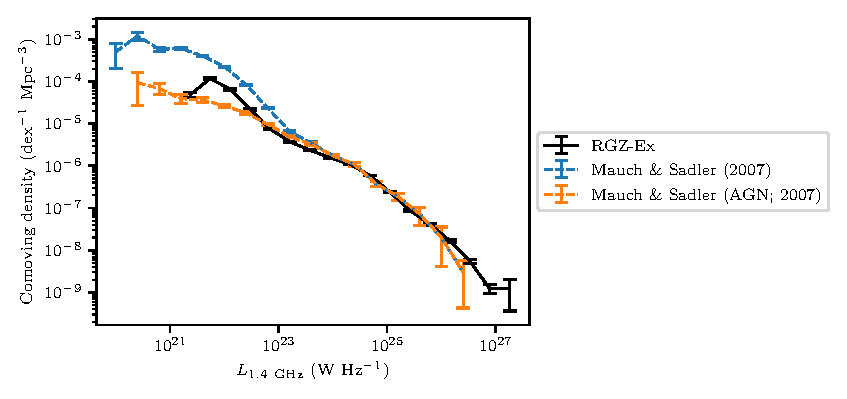
\includegraphics{rlf-images/rlf.pdf}
    \caption{RGZ-Ex radio luminosity function compared with the RLFs of \citet{mauch07rlf}.
      \label{fig:rlf}}
  \end{figure}

  In this section we present our radio luminosity functions (RLFs) derived
  from the RGZ-Ex catalogue. To calculate each RLF we 
  followed the $1/V_{\max}$ method \citep{schmidt1968vmax}. This method accounts for the effects of Malmquist bias, which is a systematic bias against sources at greater distances. We
  describe this approach in \autoref{sec:rlfs-rlf-desc}. We limit our sample to radio sources with
  \unit{1.4}{\giga\hertz} integrated flux density of at least \unit{2}{\milli Jy}
  associated with host galaxies brighter than magnitude 17 at
  \unit{3.4}{\micro\meter}, a spectroscopic redshift $0.02 \leq z \leq 0.6$,
  and an $i$-band magnitude $<20$. We chose these
  limits based on the distribution of redshifts and infrared magnitudes as well as the sensitivity of FIRST. We then remove sources with unusually high or low W1 magnitude for their redshift (more than 3 standard deviations from the mean) because many such sources have incorrect spectroscopic redshifts, e.g. blazars. There are \nsourcesrlf{} sources matching all criteria. We assume a spectral index of $\alpha = -0.7$ \citep[as is common in literature, e.g.][]{condon02radio} with flux density $f \propto \nu^{\alpha}$ where $\nu$ is the frequency. We calculate the $k$-corrected radio luminosity \citep{kochanek01kband} as follows:
  \begin{equation}
      \label{eq:luminosity}
      L = \frac{4\pi f d^2}{1+z}{(1+z)^{-\alpha}}
  \end{equation}
  where $z$ is redshift and $d$ is luminosity distance (a function of $z$).
  Uncertainties in comoving density are estimated as described in \autoref{sec:rlfs-rlf-desc}. Completeness estimates are shown in \autoref{sec:rlfs-completeness}. We discuss biases in our methods and results in \autoref{sec:rlfs-bias}.

  We compare our RLFs with \citet{mauch07rlf}, who estimated RLFs from 7~824
  manually cross-identified radio sources in the NRAO VLA Sky Survey \citep[NVSS;][]{condon98nvss}.
  Their RLFs were split into AGN and star-forming radio sources. While we
  do not make this split explicitly in our catalogue, we expect both RGZ-Ex
  and RGZ to be dominated by AGN due to the selection criterion of being extended in the selected redshift volume. We note that the redshift range used in our work, $0.02 < z < 0.6$, differs from the $0.003 < z < 0.3$ range used by \citet{mauch07rlf}.

  In \autoref{fig:rlf} we show the RLF derived from RGZ-Ex along with the RLFs from \citet{mauch07rlf}. There is good
  agreement between all three luminosity functions for luminosities greater than $10^{23}$~W~Hz$^{-1}$
  and below this luminosity the RGZ-Ex RLF is bounded above by the
  \citet{mauch07rlf} RLF. RGZ-Ex generally finds less comoving density than \citet{mauch07rlf}, which we attribute to our requirement for extent. We suggest that the peak in RGZ-Ex RLF at approximately $10^{22}$~W~Hz$^{-1}$ is due to our sample containing a small fraction of star-forming galaxies. Our criterion, however, does cut out most star-forming regions as these are often compact, which is why we report lower densities than the star-forming RLF of \citet{mauch07rlf}.

\begin{figure}
    \centering
    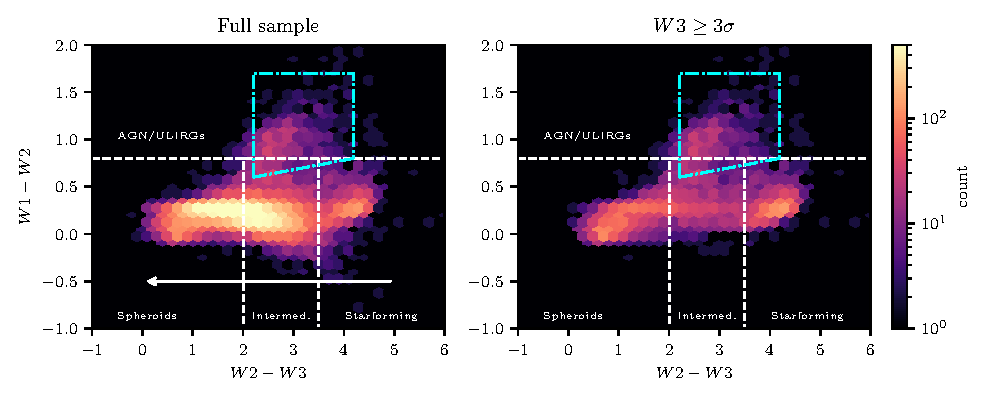
\includegraphics[width=\linewidth]{rlf-images/colour-colour.pdf}
    \caption[\emph{WISE} colour-colour distributions.]{\emph{WISE} colour-colour distributions. The dashed grey lines show
      simple host galaxy class divisions from \citet{jarrett17wise}. These
      classes are labelled in the plot. The blue dot-dashed line shows
      the empirical optical/infrared AGN criteria from \citet{jarrett11wise}. The arrow shows the direction that galaxies would shift with fainter $W3$ magnitudes. The right plot limits the sample to only sources with $W3 \geq 3 \sigma$.
      \label{fig:colour-colour}}
  \end{figure}

  \begin{figure}
      \centering
    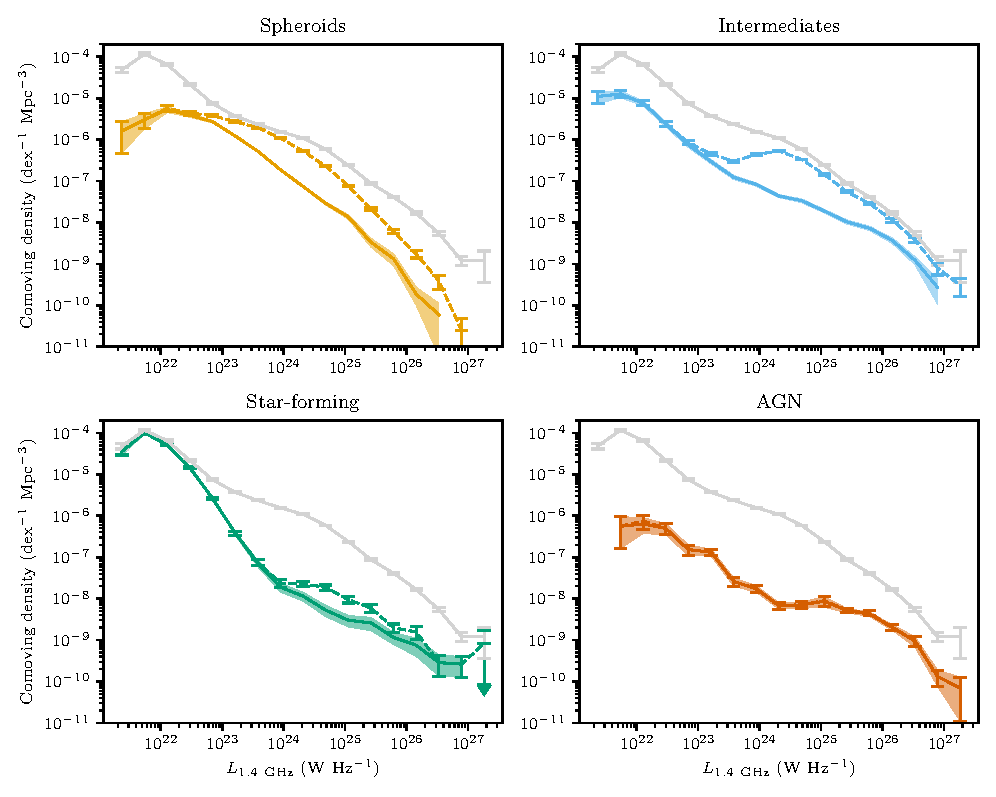
\includegraphics[width=\linewidth]{rlf-images/frlf-ir-colours.pdf}
    \caption[RLFs split by \emph{WISE} colour regions.]{RLFs split by host galaxy
      location in the \emph{WISE} colour-colour plot (\autoref{fig:colour-colour}),
      using our automated cross-identifications. The grey line is the
      total RLF for all sources. Solid lines have good $W3$ detections and dashed lines include $W3$ with low signal-to-noise.
    \label{fig:fractional-rlf}}
  \end{figure}

      The \emph{WISE} colour-colour plot, shown for RGZ-Ex in
      \autoref{fig:colour-colour}, is often used to categorise galaxies at different evolutionary stages into
      four mid-infrared colour regions that are typically populated by 1)
      spheroidals or elliptical galaxies; 2) quasi-stellar objects (QSOs),
      Seyferts or powerful AGN; 3) starbursting or luminous infrared galaxies
      (LIRGs); and 4) the intermediate region where the other three regions
      overlap. The horizontal axis, $W2-W3$, separates early- and late-type galaxies, with the star-forming late-type galaxies appearing redder (further to the right) \citep{wright10wise}. The vertical axis, $W1-W2$, separates inactive galaxies from AGN
      with strongly radiating accretion discs \citep{sadler14radio}. In
      \autoref{fig:fractional-rlf} we show the radio luminosity function split
      by host galaxy location in the mid-infrared colour-colour plot as defined by \citet{jarrett17wise}.

      Many sources have $W3$ detections with low signal-to-noise, limiting our ability to subdivide our sample. We plot both the RLFs for the sample with only $W3 \geq 3 \sigma$ as well as the RLFs for the full sample in \autoref{fig:fractional-rlf}. For the full sample we use the lower magnitude limit from All\emph{WISE} as the $W3$ magnitude (which is an upper flux limit). Using the upper flux limit as the real $W3$ flux has the effect of increasing $W2 - W3$ compared to a real detection, so objects appear further to the right of the colour-colour diagram (\autoref{fig:colour-colour}) than they ought to. This means that due to $W3$ limits, objects that should be in the spheroid set will appear in the intermediate and star-forming sets, and objects from the intermediate set will appear in the star-forming set.

      At low luminosities, our extended source RLF is dominated by galaxies with infrared
      colours consistent with star formation. The fraction
      of the RLF composed of the star-forming set drops off rapidly for
      $L_{1.4\ \mathrm{GHz}} > 10^{22}$~W~Hz$^{-1}$, as expected for galaxies with radio emission
      dominated by star formation \citep[e.g.][]{mauch07rlf}. However, the RLF slope flattens out again beyond $10^{24}$~W~Hz$^{-1}$, suggesting a second source population. This population has many missing $W3$ measurements, and these are likely intermediates or spheroids incorrectly included in the star-forming set. We therefore suggest that the
      low-luminosity RGZ-Ex sample mostly contains nearby galaxies with radio
      emission due to star formation, which appear extended in FIRST as they
      are close enough for FIRST to resolve their
      disc (greater than 20~kpc at $z = 0.2$). The remaining fraction of star-forming sources found by
      \citet{mauch07rlf}, shown in
      \autoref{fig:rlf}, would not be resolved in FIRST, as they are small or
      distant.

      Spheroids, which are hosts in the mid-infrared region corresponding to ellipticals and stars \citep{wright10wise}, comprise the majority of radio galaxies at $10^{23}$~W~Hz$^{-1}$,
      and have a peak density at $10^{22}$~W~Hz$^{-1}$. The common host galaxies for radio-loud AGN tend to be passively-evolving spheroids. It is not surprising that they are more common than star-forming galaxies at luminosities greater than $10^{22}$~W~Hz$^{-1}$. Above
      $10^{25}$~W~Hz$^{-1}$ they are less common than intermediate galaxies and
      their contribution to the luminosity function drops rapidly. This is likely due to the loss of $W3$ detections moving spheroids into the intermediate set, and we hypothesise that with deeper $W3$ observations spheroids may dominate above $10^{25}$~W~Hz$^{-1}$.

      Sources with hosts in the mid-infrared AGN region of the colour-colour diagram (\autoref{fig:colour-colour}) make
      up the smallest contribution to the radio luminosity function. They have
      a steadily decreasing density from their lowest observed $L_{1.4\ \mathrm{GHz}}$ of $10^{22}$~W~Hz$^{-1}$ to their highest of
      $10^{27}$~W~Hz$^{-1}$, but are present in all luminosity bins except for
      the very lowest. This is a set with a very low fraction of spectroscopic SDSS matches for the \emph{WISE} host galaxies. 26 per cent of
      hosts outside the \emph{WISE} AGN region have an SDSS match, compared to just 12 per
      cent of hosts inside the \emph{WISE} AGN region. This is likely due to the incomplete sampling of QSOs in the SDSS spectroscopic survey or redshift evolution effects \citep{strauss02sdss}. The fraction of the RLF contributed by galaxies classed as mid-infrared AGN increases above $10^{25}$~W~Hz$^{-1}$, meaning that high-luminosity radio AGN are also more likely to be infrared AGN than at lower radio luminosities. Note that the AGN set is unaffected by missing $W3$ detections, as the AGN set is based only on $W1-W2$.

      Galaxies residing in the intermediate mid-infrared colour region can be
      populated by both early- and late-type galaxies, which have a mix of
      processes occuring within them. These `intermediate sources' dominate in
      most luminosity ranges, and above $10^{24}$~W~Hz$^{-1}$ they comprise the
      vast majority of our sample. As intermediate-type galaxies fall between
      star-forming galaxies and passive ellipticals on the mid-infrared colour-colour plane, they do
      not have a clear morphological class and are composed of overlapping subsets of sources. The most luminous radio AGN are almost entirely found in
      this set of galaxies. In fact, as radio luminosity increases the density
      fraction shifts from spheroids toward intermediate galaxies, likely due to missing $W3$ moving objects from the spheroid set into the intermediate set.

      \begin{figure}
          \centering
        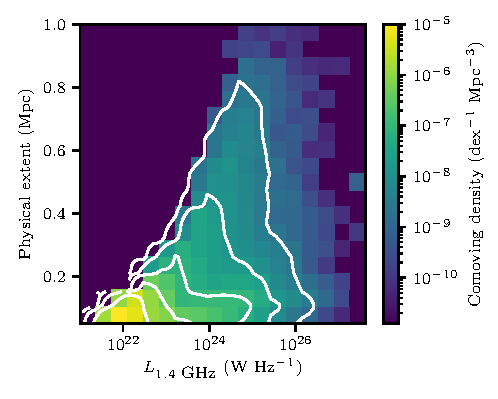
\includegraphics{rlf-images/physical-extent.pdf}
        \caption[Bivariate radio luminosity function showing radio luminosity against projected physical extent.]{Bivariate radio luminosity function showing radio luminosity against projected physical extent. Contours are on a log scale, starting at the median and increasing by 10 per cent per contour.
        \label{fig:fractional-rlf-extent}}
      \end{figure}

      In \autoref{fig:fractional-rlf-extent} we show the radio luminosity
      function for different ranges of projected physical extent of their radio emission. We estimate the angular extent as the angular distance between the most separated components in a multi-component source. This result is complementary to other Radio Galaxy Zoo studies on the effect of the environment on the size and asymmetry of the observed extended radio emission \citep{rodman19asymmetry,garon19bending}.


\section{Discussion}\label{sec:rlfs-discussion}

  \subsection{Biases and uncertainties}
    \label{sec:rlfs-bias}

    Biases enter our work due to our chosen samples and methods. Our training set,
    RGZ, is biased toward sources smaller than $1.5'$ and limited above by $\sqrt{2}
    \times 3'$ due to the $3' \times 3'$ cutout size of the RGZ user
    interface. RGZ volunteers preferentially select host
    galaxies that are brighter in $W1$, so we expect RGZ to overrepresent
    the number of sources with $W1$-bright host galaxies.

    These biases may affect our
    trained algorithm: for example, the overabundance of $W1$-bright host
    galaxies in RGZ may cause our algorithm to be less accurate when
    unassociated bright galaxies are in the field of view. Without knowing the true
    distribution of host galaxies, however, it is difficult to quantify the
    effect of such biases on our trained method.

    FIRST itself is also biased. \citet{helfand15first} describe several reasons why FIRST flux may be systematically underestimated. Most of these effects are insignificant for extended objects in our sample or are corrected in the FIRST catalogue from which we draw our flux information. The exception is the `resolving out' of diffuse and low surface brightness radio emission by the Very Large Array in its B configuration. This means that we lose flux on most nearby radio galaxies (especially those with very
    diffuse components) and may miss diffuse or dim radio galaxies entirely.
    More diffuse radio galaxies such as Fanaroff-Riley type I \citep[FRI;][]{fanaroff1974} galaxies tend to
    be toward the low end of the radio-loud luminosity distribution, about
    $10^{23}$~W~Hz$^{-1}$ \citep{best09radio}, so we expect that losing
    diffuse sources would lower our estimates of density around this
    luminosity. Large, extended lobes such as those associated with Fanaroff-Riley type II \citep[FRII;][]{fanaroff1974} galaxies may also be resolved out, so by the same mechanism we expect to lose an increasing amount of flux with increasing source angular size. This effect is compounded by flux loss at 1.4~GHz associated with synchrotron losses and adiabatic expansion losses \citep{blundell99doubles}.

    Our host galaxy redshifts may be biased. Incorrectly identifying the host galaxy may introduce sources with incorrect redshifts into the RLF, an effect which will be dominated by misidentifying galaxies as hosts where the true host is not detected. Since we are matching to optical spectra in SDSS to find
    redshifts, we are biased toward brighter host galaxies that are more
    likely to have such spectra. Without an optically-complete sample ---
    currently impossible on such scales---this effect is unavoidable.
    Brighter optical sources appear at lower redshifts, so we likely
    undersample higher-redshift (and hence higher-luminosity) galaxies.

    Our requirement for radio emission to be extended will miss radio galaxies that would be resolved and extended if they were not aligned with the line of sight. We therefore must be underestimating the population of extended sources (though assuming a random distribution of orientations, the majority of galaxies will not be aligned close to the line of sight). The requirement for extended radio emission will also impose a lower limit on linear size, which will vary with redshift: at $z = 0.6$ the effect will be strongest and we will see no sources with linear size under $33.5$ kpc. This will cause us to underestimate the population of radio galaxies with linear sizes between $10$--$30$ kpc. On the other hand, we have likely avoided significant overestimation of radio luminosity due to relativistic beaming, since we filter out sources aligned along the line of sight.

    We have estimated uncertainties in our RLF from Poisson noise in the histogram bins. We
    have likely underestimated these uncertainties as it is difficult to
    estimate uncertainty in our algorithm, though in future we anticipate that we can
    employ an ensemble of classifiers to estimate this \citep[e.g.][]{lakshminarayanan17uncertainty}.

  \subsection{Extended radio galaxies in the low-$z$ Universe}

      Our total RLFs are consistent with the idea that large, extended radio sources are typically hosted by massive ellipticals \citep{best05agn}. These RLFs match existing RLFs such as that of \citet{mauch07rlf}, except at radio luminosities below $10^{22}$~W~Hz$^{-1}$. This is unsurprising since we employ a requirement for extended emission, and, besides very nearby star-forming galaxies, FRII comprise most of the population of extended radio objects. The fractional RLF split by mid-infrared colour, \autoref{fig:fractional-rlf}, shows that spheroids reach peak density at a radio luminosity associated with a drop in density of intermediates, and intermediates begin to dominate the RLF as the spheroid density drops. Together, these mid-infrared classes of galaxy form the bulk of the extended radio galaxy RLF.

      We see a significant star-forming population in our extended sample, which means that we are likely resolving some discs in radio. While the 1/$V_{\max}$ method ensures that our RLFs account for similar galaxies throughout the Universe, even though we only resolve very nearby discs, some of the star-forming population is not included. The difference between our RLF and existing RLFs must be due to the latter containing low-luminosity sources that are compact even when very nearby.

      Can we use our RLFs to estimate the kinetic energy contribution of AGN to the galaxy halo and beyond? The extended population of AGN will be the population that contributes most mechanical energy: the major part of the energy in the jet expands the radio lobes, drives shocks or is stored in the jet magnetic field, rather than being emitted as radiation \citep{godfrey16power, hardcastle14lobes}. Extended radio sources should therefore represent the bulk of AGN feedback: radio galaxies with extended jets will inject mechanical energy out to larger distances from the core of the host galaxies than those with smaller jets. This is supported by e.g. \citet{turner15agn}, who found that extended sources comprised the bulk of the mechanical energy contribution. By assuming a relationship between radio luminosity and radio jet mechanical energy, we can use our extended source RLFs to estimate the contribution of extended AGN to energy in the intergalactic/circumgalactic medium (IGM/CGM). But assuming such a relationship is not without problems: the radio lobe luminosity experiences significant evolution \citep[e.g.][]{bicknell97css}, the surrounding IGM/CGM may interact with the radio lobe expansion in non-trivial ways \citep[e.g.][]{hardcastle13lobes} and the relationship between the mechanical energy and radio luminosity has high scatter on individual radio sources \citep{hardcastle13lobes}. With our sample size, these effects should be diminished, and with these caveats in mind we will estimate the energy contribution of extended sources to the IGM. We assume a scaling relation of $\ln Q = \beta \ln L_\nu + Q_0$, where $Q$ is the jet power and $L_\nu$ is the monochromatic radio luminosity at frequency $\nu$. The values for $\beta$ and $Q_0$ vary significantly across the literature, based on different physical assumptions and samples. \citet{willott99radio} presented a widely-used relationship
      \begin{equation}
        \ln Q = \ln (f^{3/2} 3 \times 10^{38}) + \frac{6}{7} \ln \left[\frac{L_{151~\mathrm{MHz}}}{10^{28}~\mathrm{W\ Hz}^{-1}}\right],
      \end{equation}
      with a scaling constant $1 \leq f \leq 20$ and $Q$ in watts. Other models exist with different slopes, e.g. \citet{birzan08power} suggest that $\beta \approx 0.5 - 0.7$ and \citet{cavagnolo10relation} find $\beta \approx 0.7$. \citet{shabala13power} show that the scalings presented by \citet{willott99radio} are consistent with independent theoretical modelling for high-power radio galaxies. \citet{godfrey16power} on the other hand provide a summary of the literature in this field and suggest that these correlations are from mutual distance dependence rather than intrinsic relationships. They find that there is no strong empirical evidence for such a correlation in either FRI or FRII. However, their theoretical models suggest $\beta \approx 0.5,0.8$ for FRI and FRII respectively, which is consistent with \citet{willott99radio}. The relationship between luminosity and kinetic energy is not yet settled, but we can still use this popular scaling method both to explore the consequences of our RLFs and for comparison with previous work.

      Scaling the frequency to $1.4$~GHz, and assuming a spectral index of $\alpha = -0.7$, $\beta = 6/7$, and $Q_0 = \ln (f^{3/2}) + 89.9$, we can write the \citet{willott99radio} relation as
      \begin{equation}
        \ln (Q) = \ln (f^{3/2}) + 89.9 + \frac{6}{7} \ln \left[\frac{L_{1400~\mathrm{MHz}}}{10^{28}~\mathrm{W\ Hz}^{-1}}\right].
      \end{equation}
      Assuming $f \in [1, 20]$ gives $Q_0 \in [89.9, 94.4]$. Integrating over our RLF we find $Q \in [1.3 \times 10^{30}, 1.2 \times 10^{32}]$~W~Mpc$^{-3}$. This is likely a lower limit as we are missing extended radio sources oriented along our line-of-sight and nearby diffuse extended radio sources (e.g. FRI), and \citet{shabala18plane} argues that many `compact' AGN may in fact be extended but below the sensitivity of surveys such as FIRST. Our results are consistent with other literature \citep[e.g][who estimated the energy contribution as $7 \times 10^{31}$ W~Mpc$^{-3}$]{hardcastle19rlagn}. 

  \subsection{Future work}

    With such a large sample size, further partitioning of the RLF into subsamples is possible. Any combination of the features investigated here, plus further host galaxy and radio properties, could be used to generate fractional RLFs. Automated classifiers such as \texttt{ClaRAN} \citep{wu19claran} or feature extractors such as \texttt{PINK} \citep{polsterer15pink,galvin19som,ralph19ae} could provide a way to divide the RLF by radio morphology. These methods provide a way of dividing galaxy classes based directly on the radio image, rather than the host galaxy like we have done here, and so should not be affected by extinction or redshift in the same way as our sample. Such subsamples would lend insight into how radio power is connected to radio morphology and generation mechanisms. Cross-matching with other surveys such as NVSS or the 150~MHz TIFR GMRT Sky Survey would provide properties such as the spectral index and observations of diffuse emission missed by FIRST \citep[as used by][]{kimball08}. Such properties could also be used to create interesting and insightful fractional RLFs.

    While we have not investigated the link between extended sources and their local environments, this will be the focus of future work. Environment will heavily factor into the source sizes, morphologies, and so on, following work such as \citet{rodman19asymmetry} and \citet{garon19bending}.

    Ongoing radio surveys such as EMU, VLASS \citep{lacy20vlass}, and LoTSS \linebreak \citep{shimwell19lotss} will greatly increase the number of extended sources. However, our sample size limitations in this chapter are not from FIRST, but from SDSS: until next-generation spectroscopic surveys are available, redshifts will be the limiting factor. To significantly increase our sample size would require much greater numbers of redshifts.

\section{Summary}\label{sec:rlfs-summary}

  Extended radio sources provide an opportunity to study the interaction between AGN and their large-scale environments. We trained the binary cross-identification method on the Radio Galaxy Zoo to generate the largest sample of reliably cross-identified, extended radio sources, and this large sample allows us to investigate their bulk distributions in new, detailed ways. We estimated radio luminosity functions split by mid-infrared colour, physical extent and redshift. Despite our extendedness criterion, we found a significant star-forming population. We estimated that extended AGN contribute between $1.3 \times 10^{30}$ and $1.2 \times 10^{32}$~W~Mpc$^{-3}$ of mechanical energy to their environment. Ongoing and future surveys such as EMU will provide even greater numbers of extended radio sources, and our combination of machine learning and astronomy methodology will allow these samples to be cross-identified and investigated efficiently and reliably.

\section{Acknowledgements}

This publication has been made possible by the participation of more than
11~000 volunteers in the Radio Galaxy Zoo project. Their contributions are
individually acknowledged at \url{http://rgzauthors.galaxyzoo.org}. Radio
Galaxy Zoo makes use of data products from the \emph{Wide-field Infrared Survey
Explorer} and the Very Large Array. The \emph{Wide-field Infrared Survey Explorer}
is a joint project of the University of California, Los Angeles, and the Jet
Propulsion Laboratory/California Institute of Technology, funded by the
National Aeronautics and Space Administration. The National Radio Astronomy
Observatory is a facility of the National Science Foundation operated under
cooperative agreement by Associated Universities, Inc. The figures in this
work made use of Astropy, a community-developed core Python package for
Astronomy \citep{astropy}. Partial support for this work for L.R. and A.F.G. comes from National Science Foundation grant AST-1714205 to the University of Minnesota. H.A. benefited from grant CIIC 218/2019 of Universidad de Guanajuato. M.A. and A.T. were supported by the Australian Government Research Training Program. We thank J.~Nabaglo and A.~Gruen for their help with efficient data preprocessing. We thank H.~Zovaro, T.~J.~Galvin and H.~Tang for their comments on the draft of this chapter.

